%\chapter{Implementation}\label{s:implementation}
%\graphicspath{ {./images/} }
%\begin{figure}[t]
%\centering
%\caption{Zoomed in on QAS of ASR-1}
%\label{fig:ASR2}
%\end{figure}
%\includegraphics[width=12cm]{Decomposition of ASR and QAS_zoomed in on %ASR-1 and ASR-2_v2.jpg}\\
\chapter{Implementation}\label{s:Implementation}
\todo{better describe why there is a different between currently implemented and future architectures}
Research question 3 focuses on patterns and tactics, in context of software architecture. Bass \etal \cite{Bass2015SoftwareAI} describes architectural patters as "Compositions of architectural elements and provide packaged strategies for solving some of the problems facing a system." This section will give examples on patterns and tactics, combined with trade-offs to take in account when designing a system. Combined with the collected business goals and concerns.

Patterns exist of multiple tactics. While tactics are chosen to empower a single quality attribute, a pattern could serve multiple quality attributes. This chapter will cover one pattern and a set of tactics. Both focused on the quality attribute 'Confidentiality'.

Section \ref{QI} discusses the quantified problem and argues logical reasoning will define how a solution could mitigate the operational problem mentioned in section \ref{Operational_problem}
\section{Pattern - Zero-knowledge proof}
%\graphicspath{ {./images/} }
%\begin{figure}[t]
%\centering
%\label{fig:ZKP}
%\includegraphics[width=15cm]{A zero-knowledge-proof-based %digital identity management scheme in blockchain.png}\\
%\caption{Zero knowledge proof}
%\end{figure}
By definition of Goldwasser \etal \cite{Goldwasser} "A zero-knowledge proof (ZKP) makes it possible to prove a statement is true while preserving confidentiality of secret information". 
Xiaohui Yang and Wenjie Li \cite{YANG2020102050} state "Zero-knowledge proof (ZKP) is a cryptography technique, which means that the prover can convince the verifier that a certain statement is correct without providing the verifier with any additional information or leaking any information about the witness." Figure \ref{fig:ZKP_usecase} shows a schema on how this principle works. The ZKProof Community reference \cite{2019:zkproof:community-reference-0.2} of Bennarroch \etal is intended to provide a reference for development of zero-knowledge proof by contribution of world-renowned cryptographers, practitioners and industry leaders.
Reasoning why this methodology or pattern is a solution for the operational problem in section \ref{OP} is if there is no identity data to be shared or replicated, there will be no profiling or unauthorized correlation of identity data can be done. Without identity data it's not possible to commit identity fraud.

\subsection{Application of Zero-Knowledge proof}
Zero-knowledge proof itself is a methodology which translates in a variety of technical implementation possibilities. Assessing suitability of this pattern is done by scoping a possible solution in a use-case.

\todo{Improve this use-case description}
Acting parties: Employer, employee, Belastingdienst.
When a citizen starts working at an employer, the employer is responsible for the wage declaration. The wage declaration contains income taxes and it's transferred to the tax authorities. In the happy flow, all information off the employee is processed correctly. However, there are practical exceptions, where an employer receives the wrong BSN. The BSN is incorrect or does not match with the employee. Both result in overhead in administration and incorrect data within wage declaration chain.
A possible solution would be to let the employer check the correctness of personal information when hiring a citizen. Section \ref{BRP} describes the BRP as the central database of personal identity data of citizens and could be used for this purpose. However, giving all employees access to this source of data is not desirable. Not acting in good faith could result in scraping the database to commit fraud or unauthorized usage of personal data, like mentioned in section \ref{Operational_problem}. Zero-knowledge proof could be a pattern that can resolve this problem by providing a check if the data the employer receives from an employee matches with a person in the BRP. 

\graphicspath{ {./images/} }
\begin{figure}
\centering
\label{fig:ZKP_usecase}
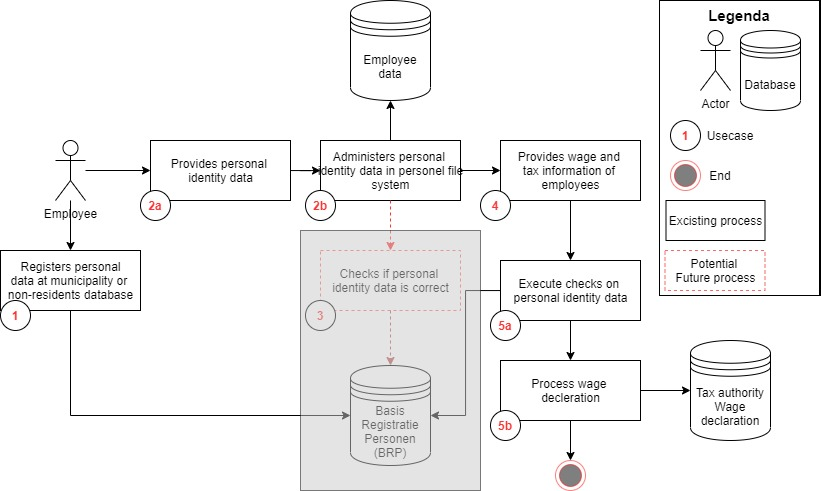
\includegraphics[width=17cm]{Usecase for zkp.jpg}\\
\caption{Example usecase where ZKP could suffice}
\end{figure}

\todo{Add solution, what to take into account globally}

\subsection{Trade-offs and concerns}
\todo{Scrapbook, needs refinement}
Maintainability - The complexity of the methodology and need of a continuous maintenance on the part of applying the correct algorithm. 
Adaptability - 

Depending on the type of algorithm used, it's up-to-date on known issues and treats (bedreigingen).
Trade-off snelheid/efficientie. Depends on choosen methodology and algoritm. It's needed to address the needed calculation power (and assumed costs) when selecting algoritms 
\todo{Better describe and support these trade-offs and concerns}

\section{Tactics - Quality attribute 'Confidentiality'}
\graphicspath{ {./images/} }
\begin{figure}
\centering
\label{fig:Tactics}
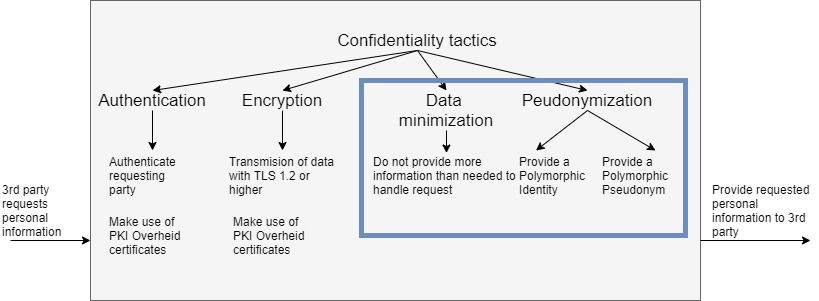
\includegraphics[width=17cm]{Tactics.jpg}\\
\caption{Confidentiality tactics}
\end{figure}

\subsection{Authentication}
A commonly used method for authentication purposes is usage of a certificate. For parties who communicate with on or on behalf of the Dutch government the government issues PKIoverheid (PKIO) certificates. These certificates are used for Authentication, Electronic signatures and encryption. \cite{Logius_PKIO}

\subsection{Data minimization}
\todo{add a description of this method, but emphasise how it's possible to use in software architecture}
\lipsum[1-1]

\subsection{Encryption - Transfer of data is encrypted with TLS 1.2 or higher}
A broadly implemented standard. The Dutch government has a reference architecture NORA (Nederlandse Overheid Referentie Architecture) \cite{NORA} which states this standard needs to be applied or otherwise explained why it has not been implemented \cite{NORA_PasToeOfLegUit}. On the part of TLS its clear version 1.2 or higher is accepted, but version 1.3 is prefered \cite{NORA_TLS}. 

\subsection{Peudonymization - Polymorphic Identity or Polymorphic Pseudonym}
When it's mandatory to share personal information, because it's for example mandatory by law, it's possible to provide this information as a pseudonym. GDPR \cite{GDPR} defines this method as a possibility to mitigate unwanted disclosure of personal information. 
This technique is already implemented and proven it can work by Erik Verheul \cite{VerheuleID}.


%%% Local Variables:
%%% mode: latex
%%% TeX-master: "../thesis"
%%% End:
